\documentclass[slidestop,compress,11pt,xcolor=dvipsnames,french]{beamer}
\usefonttheme[onlymath]{serif}
\definecolor{LHCblue}{RGB}{204, 0, 0}
\usecolortheme[named=LHCblue]{structure}
\usepackage[french]{babel}
\usepackage[utf8]{inputenc}
\usepackage[bars]{beamerthemetree} % Beamer theme v 2.2
\usepackage{movie15}
%\usepackage{kerkis}
\mode<presentation>
\newcommand*\oldmacro{}%
\let\oldmacro\insertshorttitle%
\renewcommand*\insertshorttitle{%
  \oldmacro\hfill%
  \insertframenumber\,/\,\inserttotalframenumber}
\setbeamertemplate{footline}[frame number]
%~~~~~~~~~~~~~~~~~~~~~~~~~~~~~~~~~~~~~~~~~~~~~~~~~~~~~~~~~~~
\setbeamercovered{dynamic}
\usetheme{Ilmenau} % Beamer theme v 3.0
\useoutertheme[subsection=true]{smoothbars}%Beamer Outer Theme-circles on top

\useinnertheme{circles} %rectangle bullet points instead of circle ones
\beamertemplatenavigationsymbolsempty

%~~~~~~~~~~~~~~~~~~~~~~~~~~~~~~~~~~~~~~~~~~~~~~~~~~~~~~~~~~~~~~~~~~~~~
\title[Flyway 101]{Flyway 101}
\author[Lunch and Learn]{\Large Lunch and Learn}
\date[Septembre 2020]{\normalsize
\begin{center}
\parbox{0cm}{\begin{tabbing}
\hspace*{2cm}\= \kill
Auteur :\> Said Mezghanni
\end{tabbing}}
\end{center}
}
\institute{L'équipe du PaaP}

%~~~~~~~~~~~~~~~~~~~~~~~~~~~~~~~~~~~~~~~~~~~~~~~~~~~~~~~~~~~~~~~~~~~~~~~~~~~~~~~~~~
\usepackage{tikz}
\usepackage{multicol}
\usepackage{lmodern}
\usepackage{lipsum}
%\usepackage{graphicx}
\usepackage{marvosym}
%------------------tikz------------------------

\usetikzlibrary{%
calc,%
fadings,%
shadings%
}

\usetikzlibrary{arrows,snakes,shapes}
\let\otp\titlepage
\renewcommand{\titlepage}{\otp\addtocounter{framenumber}{-1}}

%%%%%%%%%%%%%%%%%%%%%%%%%%%%%%%%%%%%%%%%%%%%%%%%%%%%%%%%%%%%%%%%%%%%%%%%%%%%%%%%%%%%%%%%%%%%%%%%%%%%%%%%
\begin{document}
\begin{frame}[plain]
\titlepage
\end{frame}
%%%%%%%%%%%%%%%%%%%%%%%%%%%%%%%%%%%%%%%%%%%%%%%%%%%%%%%%%%%%%%%%%%%%%%%%%%%%%%%%%%%%%%%%%%%%%%%%%%%%%%%%
\setcounter{framenumber}{0}
\begin{frame}
  \frametitle{Plan}

  \tableofcontents
\end{frame}
%%%%%%%%%%%%%%%%%%%%%%%%%%%%%%%%%%%%%%%%%%%%%%%%%%%%%%%%%%%%%%%%%%%%%%%%%%%%%%%%%%%%%%%%%%%%%%%%%%%%%%%%
\AtBeginSection[]
{
  \begin{frame}<beamer>
    \frametitle{Plan}
    \tableofcontents[currentsection]
  \end{frame}
}
%%%%%%%%%%%%%%%%%%%%%%%%%%%%%%%%%%%%%%%%%%%%%%%%%%%%%%%%%%%%%%%%%%%%%%%%%%%%%%%%%%%%%%%%%%
% Introduction
%%%%%%%%%%%%%%%%%%%%%%%%%%%%%%%%%%%%%%%%%%%%%%%%%%%%%%%%%%%%%%%%%%%%%%%%%%%%%%%%%%%%%%%%%%
\section{Introduction}
\subsection*{Flyway}
\begin{frame}

Flyway est un outil open-source de migration de base de données \\ 
Le projet a commencer avec une première release en 2010. \\

\vspace{1cm}
\textbf {L'outil est disponible sous trois éditions:  \\}
    \begin{itemize}
        \item Community Edition
        \item Pro Edition 
        \item Enterprise Edition
    \end{itemize}
\end{frame}
\subsection*{Outils fournis par Flyway}
\begin{frame}
\setbeamertemplate{itemize/enumerate body begin}{\footnotesize}
\vspace{1cm}
\textbf {Liste des outils offert par Flyway: \\}
    \begin{itemize}
        \item Command-line: permet d'executer Flyway en ligne de commande utile pour les agents Docker.
        \item Maven-plugin: permet d'executer Flyway dans un build Maven.
        \item Gradle-plugin: permet d'executer Flyway dans des tasks Gradle.
        \item Java-API: permet d'executer Flyway a l'interieur de code Java.
        \item Plugins communautaire: npm, Jenkins, SpringBoot, Quarkus,...
    \end{itemize}
\end{frame} 

\subsection*{Configurations des outils}
\begin{frame}
\setbeamertemplate{itemize/enumerate body begin}{\footnotesize}
\vspace{1cm}
\textbf {Il est possible de configurer les outils Flyway par plusieurs manière: \\}
    \begin{itemize}
        \item variables d'environnements 
        \item fichier de config: flyway.conf
        \item fichier de config par migration: myscript.sql.conf 
        \item placeholders: permet de faire du templating sur les scripts de migrations suivant des paramètres prédéfinis
        \item config SSL: il faut injecter des certificats dans le formats Java (keystore et truststore) a la JVM ou Flyway va s'executer puis configurer la connexion a la BD pour enforcer le ssl.
    \end{itemize}
\end{frame} 

\subsection*{Base de données supportés}
\begin{frame}
\setbeamertemplate{itemize/enumerate body begin}{\footnotesize}
\vspace{1cm}
\textbf {Liste des bases de données supportés: \\}
    \begin{itemize}
        \item Oracle (incl. Amazon RDS)
        \item MySQL (incl. Amazon RDS, Azure Database \& Google Cloud SQL)
        \item MariaDB (incl. Amazon RDS)
        \item SQL Server (incl. Amazon RDS \& Azure SQL Database)
        \item PostgreSQL (incl. Amazon RDS, Azure Database, Google Cloud SQL \& Heroku)
        \item et plein d'autres base de données...
    \end{itemize}
\end{frame}
%%%%%%%%%%%%%%%%%%%%%%%%%%%%%%%%%%%%%%%%%%%%%%%%%%%%%%%%%%%%%%%%%%%%%%%%%%%%%%%%%%%%%%%%%%
%Fonctionnalités
%%%%%%%%%%%%%%%%%%%%%%%%%%%%%%%%%%%%%%%%%%%%%%%%%%%%%%%%%%%%%%%%%%%%%%%%%%%%%%%%%%%%%%%%%%
\section{Fonctionnalités}
\subsection*{Migrations}
\begin{frame}{Définitions}

Avec Flyway, toutes les modifications apportées à la base de données sont appelées \textbf{migrations}. \\
Les migrations peuvent être : 
\begin{itemize}
 \item versionnées
 \item répétables
\end{itemize}

Les migrations versionnées se présentent sous 2 formes:
\begin{itemize}
 \item régulière
 \item annulée
\end{itemize}

\end{frame}

\begin{frame}{Type de migrations}

\begin{itemize}
 \item \textbf{Les migrations versionnées} ont une version, une description et un checksum. La version doit être unique. La checksum permet de détecter les changements accidentels. Les migrations versionnées sont appliqués dans l'ordre une seule fois. 
 \item \textbf{Les migrations d'annulation}: en option, l'effet d'une migration régulière peut être annulé en fournissant une migration d'annulation avec la même version. 
 \item \textbf{Les migrations répétables} ont une description et un checksum, mais pas de version. Au lieu d'être exécutés une seule fois, ils sont (ré)appliqués à chaque fois que leur checksum change. 

\end{itemize}
\end{frame}

\begin{frame}{Langage de migration}
\setbeamertemplate{itemize/enumerate body begin}{\footnotesize}

Les migrations sont le plus souvent écrites en SQL. Ils sont généralement utilisées pour :

\begin{itemize}
\item Modifications DDL (CREATE/ALTER/DROP: TABLES,VIEWS,…)
\item Modifications simples des données (CRUD dans les tables)
\item Modifications simples des données en masse (CRUD dans les tables)
\end{itemize}

\vspace{1cm}

Les migrations basées sur Java ou sur des scripts Bash, Python,... (en beta) conviennent parfaitement à toutes les modifications qui ne peuvent pas être facilement exprimées à l'aide de SQL:
\begin{itemize}
 \item Modifications BLOB \& CLOB
 \item Modifications avancées des données en masse (recalculs, changements de format avancés,…)
\end{itemize}

\end{frame}

\begin{frame}{Migrations SQL/Script}
\setbeamertemplate{itemize/enumerate body begin}{\footnotesize}
Nommage :
\begin{center}
 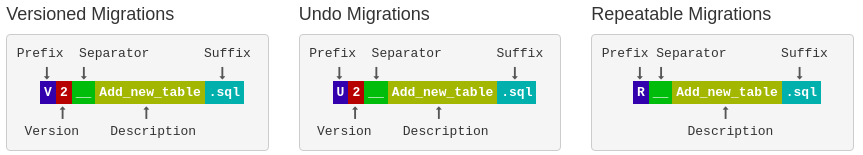
\includegraphics[scale=0.3]{nommage_sql.png}
 % nommage_sql.png: 863x155 px, 72dpi, 30.44x5.47 cm, bb=0 0 863 155
\end{center}

Emplacement des migrations :
\begin{itemize}
 \item classpath: utilisable dans les builds Java avec les plugins Maven et Gradle
 \item filesystem: utilisable avec le cli et les plugins
 \item s3/gcs: (en beta)
\end{itemize}

\begin{center}
 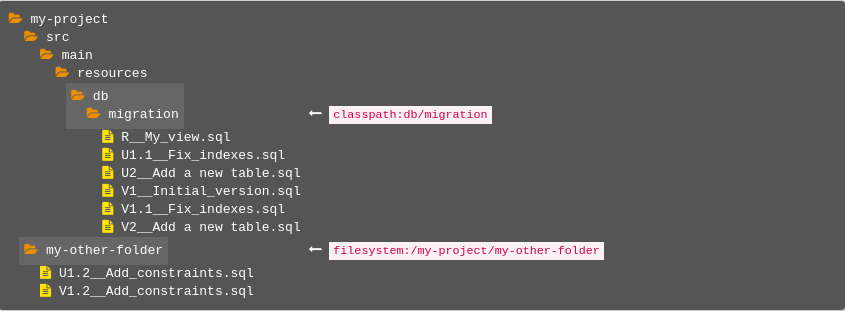
\includegraphics[scale=0.2,keepaspectratio=true]{locations_sql.png}
 % locations_sql.png: 845x312 px, 72dpi, 29.81x11.01 cm, bb=0 0 845 312
\end{center}
\end{frame}

\begin{frame}{Migrations Java}
\setbeamertemplate{itemize/enumerate body begin}{\footnotesize}
Nommage :
\begin{center}
 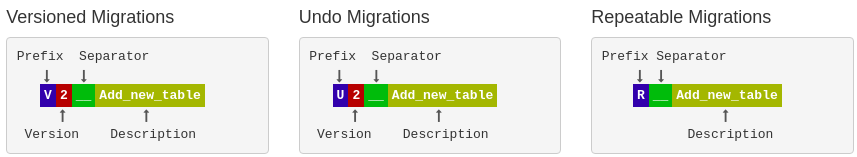
\includegraphics[scale=0.3]{nommage_java.png}
 % nommage_sql.png: 863x155 px, 72dpi, 30.44x5.47 cm, bb=0 0 863 155
\end{center}

Emplacement des migrations :
\begin{itemize}
 \item classpath: utilisable dans les builds Java avec les plugins Maven et Gradle. Il faut compiler les classes avant de lancer la migration.
\end{itemize}

\begin{center}
 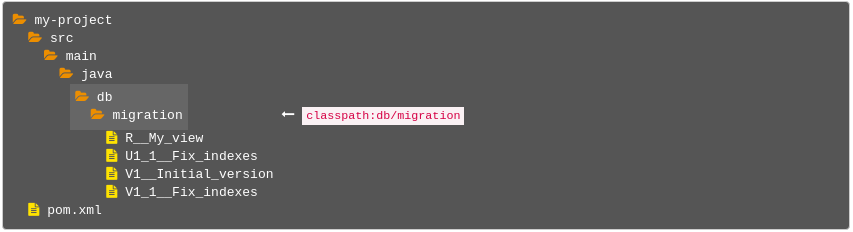
\includegraphics[scale=0.2,keepaspectratio=true]{locations_java.png}
 % locations_sql.png: 845x312 px, 72dpi, 29.81x11.01 cm, bb=0 0 845 312
\end{center}

\end{frame}

\begin{frame}{Table d'historique de schéma}
Pour garder une trace des migrations qui ont déjà été appliquées, quand et par qui, Flyway ajoute une table d'historique de schéma. Il contient également les checksum, les temps et l'état d'exécutions des migrations.
\begin{center}
 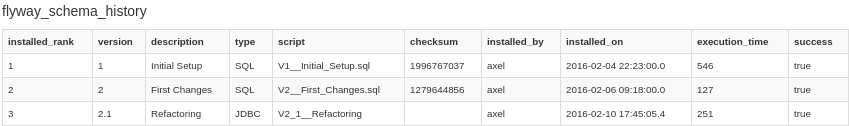
\includegraphics[scale=0.3,keepaspectratio=true]{schema_history_table.png}
 % schema_history_table.png: 849x126 px, 72dpi, 29.95x4.45 cm, bb=0 0 849 126
\end{center}

\textbf{L'aspect transactionnel:} \\
Par défaut, Flyway encapsule l'exécution de chaque migration dans une seule transaction.\\
Il est aussi possible de le configurer pour encapsuler l'exécution complète de toutes les migrations dans une seule transaction.                                                                            

\end{frame}
\subsection*{Fonctionnalités avancées}
\begin{frame}{Callbacks}
Dans certaines situations, nous avons besoins d'exécuter des actions répétitives comme la recompilation des procédures, la mise-à-jour des vues matérialisées, les taches de maintenance... \\
\vspace{1cm}
Pour ces besoins, Flyway offre la possibilité de definir des scripts de Callbacks: \\
 \begin{itemize}
  \item \textbf{en SQL}: ils sont definits de la meme maniere que les scripts de migration. Le nom du script doit correspondre a l'event écouté (beforeMigrate.sql, beforeEachMigrate.sql,...)
  \item \textbf{en Java}: il est aussi possible de programmer des Hook sur un ou plusieurs Callbacks en Java.
 \end{itemize}
\end{frame}

\begin{frame}{Error Overrides}
\setbeamertemplate{itemize/enumerate body begin}{\footnotesize}
Lors de exécutions des migrations SQL:
\begin{itemize}
\item en cas d'erreur: Flyway marque la migration comme échoué et la rollback automatiquement si possible.
 \item en cas de warning: il est retourné.
\end{itemize}

\vspace{1cm}

Avec la fonctionnalité de redefinitions des erreurs(pro et enterprise), il est possible de:
\begin{itemize}
 \item traitez une erreur comme un warning car la migration va la traitera correctement plus tard
 \item traitez un warning comme une erreur afin d'échouer rapidement et de pouvoir résoudre le problème plus tôt
 \item effectuer des actions supplémentaires lorsqu'une erreur/warning spécifique est émis 
\end{itemize}
\end{frame}

\begin{frame}{Dry Runs}
La fonctionnalité de dry-run (Pro et Enterprise) est disponible pour les migrations Java et SQL et permet de: 
\begin{itemize}
 \item prévisualiser les modifications que Flyway apportera à la DB
 \item soumettre les instructions SQL pour examen à un DBA avant de les appliquer
 \item utiliser Flyway pour générer le script de mis à jour, mais utiliser un outil différent pour appliquer les modifications
\end{itemize}
\end{frame}

\section{Commandes}
\subsection*{Commandes}

\begin{frame}{Migrate/Undo}
\setbeamertemplate{itemize/enumerate body begin}{\footnotesize}
\begin{itemize}
 \item \textbf{Migrate} : migre le schéma vers la dernière version. Flyway créera automatiquement la table d'historique de schéma si elle n'existe pas.
 \item \textbf{Undo} : annule la migration versionnée la plus récemment appliquée (pro et Enterprise)
\end{itemize}
\vspace{1cm}
Options des commandes migrate/undo (beta):
\begin{itemize}
 \item \textbf{Cherry pick}: spécifiez les migrations à appliquer avec l'option \textit{-cherryPick}. Exemple: \textit{flyway migrate -cherryPick="5,create\_view"}
 \item \textbf{Mark as applied}: avec l'option \textit{skipExecutingMigrations=true}, l'exécution du script est ignoré, en mettant à jour la table d'historique de schéma.
\end{itemize}
\end{frame}
\begin{frame}{Info/Validate}
\setbeamertemplate{itemize/enumerate body begin}{\small}
\setbeamertemplate{itemize/enumerate subbody begin}{\footnotesize}
\begin{itemize}
 \item \textbf{Validate} : valide les migrations appliquées par rapport à celles disponibles.
 \item \textbf{Info} : imprime les détails et les informations d'état de toutes les migrations. Les états possible d'une migration:
    \begin{itemize}
        \item \textbf{success}: la migration est réussit
        \item \textbf{pending}: la migration est détectée et n'est pas appliquée 
        \item \textbf{failed}: lorsque la migration échoue (BD ne supporte pas les transactions) 
        \item \textbf{undone}: la migration versionnée est annulée par la commande undo.
        \item \textbf{outdated}: la migration répétable dont la checksum a changé
        \item \textbf{futur}:  la migration versionnée appliquée a une version supérieure à la version la plus élevée connue.
    \end{itemize}
\end{itemize}
\end{frame}
\begin{frame}{Clean/Baseline/Repair}
\setbeamertemplate{itemize/enumerate body begin}{\small}
\setbeamertemplate{itemize/enumerate subbody begin}{\footnotesize}
\vspace{1cm}
\begin{itemize}
 \item \textbf{Clean}: supprime tous les objets dans les schémas configurés.
 \item \textbf{Baseline}: la commande baseline sert à introduire Flyway dans les bases de données existantes en les basant sur une version spécifique.
 \item \textbf{Repair}: répare la table d'historique de schéma en :
    \begin{itemize}
        \item supprimant les entrées de migration ayant échoué
        \item réalignant les checksum, les descriptions et les types des migrations appliquées avec les migrations disponibles
        \item supprimant les migrations repetables supprimé (beta)
    \end{itemize}
\end{itemize}
\end{frame}

%%%%%%%%%%%%%%%%%%%%%%%%%%%%%%%%%%%%%%%%%%%%%%%%%%%%%%%%%%%%%%%%%%%%%%%%%%%%%%%%%%%%%%
% %% Demo
%%%%%%%%%%%%%%%%%%%%%%%%%%%%%%%%%%%%%%%%%%%%%%%%%%%%%%%%%%%%%%%%%%%%%%%%%%%%%%%%%%%%%%
\section[Démo]{Démonstration}
\subsection*{Scenario 1}
\begin{frame}
\end{frame}
\subsection*{Scenario 2}
\begin{frame}
\end{frame}

%%%%%%%%%%%%%%%%%%%%%%%%%%%%%%%%%%%%%%%%%%%%%%%%%%%%%%%%%%%%%%%%%%%%%%%%%%%%%%%%%%%%%%
%% Discussion
%%%%%%%%%%%%%%%%%%%%%%%%%%%%%%%%%%%%%%%%%%%%%%%%%%%%%%%%%%%%%%%%%%%%%%%%%%%%%%%%%%%%%%
\section[Discussion]{Discussion et Q\&A}
\subsection*{Conclusion }
\begin{frame}
\textbf {Pros : \\}
\begin{itemize}
 \item Riche en fonctionnalités 
 \item Supporte plusieurs langage/platform/BD
 \item Facilite les taches de maintenance pour des usecases complexes
\end{itemize}
\textbf {Cons : \\}
\begin{itemize}
 \item L'édition communautaire est limité 
 \item Model de facturation par schema pour les versions payantes
\end{itemize}
\textbf {Alternatives : \\}
\begin{itemize}
 \item Liquibase 
 \item Alembic
 \item Orcas DB
 \item Dbmate
\end{itemize}
\end{frame}

\subsection*{Q\&A et Références}
\begin{frame}
\begin{center}
 
\includegraphics[scale=0.3,keepaspectratio=true]{qa.jpg}
 % qa.jpg: 560x235 px, 100dpi, 14.22x5.97 cm, bb=0 0 403 169
\end{center}

\vspace{1cm}
\begin{itemize}
 \item Documentation : \url{https://flywaydb.org/documentation/} 
 \item Blog : \url{https://flywaydb.org/blog/flyway-7.0.0-beta}
 \item FAQ : \url{https://flywaydb.org/documentation/faq}
\end{itemize}

\end{frame}

\begin{frame}[plain,noframenumbering]
\vspace{2.5cm}
\begin{center} 
\begin{beamercolorbox}[rounded=true,sep=8pt,center]{title}
   	\Huge Merci pour votre attention ! 
		\end{beamercolorbox}%
\end{center} 
\end{frame} 

\end{document}

